\documentclass{beamer}
\beamertemplatenavigationsymbolsempty
\usecolortheme{beaver}
\setbeamertemplate{blocks}[rounded=true, shadow=true]
\setbeamertemplate{footline}[page number]
%
\usepackage[utf8]{inputenc}
\usepackage[english,russian]{babel}
\usepackage{amssymb,amsfonts,amsmath,mathtext}
\usepackage{subfig}
\usepackage[all]{xy} % xy package for diagrams
\usepackage{array}
\usepackage{multicol} % many columns in slide
\usepackage{hyperref} % urls
\usepackage{hhline} %tables
\usepackage{comment} %comments

\newcommand{\btVFill}{\vskip0pt plus 1filll}
\newcommand{\secref}[1]{\autoref{#1}. \nameref{#1}}
%----------------------------------------------------------------------------------------------------------

\title[\hbox to 56mm{Получение фазовой траектории сопряженных маятников с помощью Neural ODE}]{Получение фазовой траектории сопряженных маятников с помощью Neural ODE}
\author[А. Б. Богданов]{Александр Иванович Богданов}
\institute[]{Московский физико-технический институт}
\date{\footnotesize
\par \textbf{Lab 405a}
\par\smallskip\emph{Курс:} Прогнозирование временных рядов}

%----------------------------------------------------------------------------------------------------------
\begin{document}
%----------------------------------------------------------------------------------------------------------

\begin{frame}

    \maketitle

\end{frame}

%-----------------------------------------------------------------------------------------------------

\begin{frame}{Цель работы}

    \textbf{Задача}: С помощью Neural ODE восстановить фазовую траекторию сопряженных маятников.

\end{frame}

%-----------------------------------------------------------------------------------------------------

\begin{frame}{Литература}

    \begin{enumerate}
        \item \url{https://web.archive.org/web/20230516005825/https://en.wikipedia.org/wiki/Pendulum_(mechanics)\#Coupled_pendula};

        \item \url{https://github.com/intsystems/MathematicalForecastingMethods/blob/main/seminars/seminar8.ipynb}.
    \end{enumerate}
    
\end{frame}

%-----------------------------------------------------------------------------------------------------

\begin{frame}{Постановка задачи}

    \begin{figure}
        \centering
        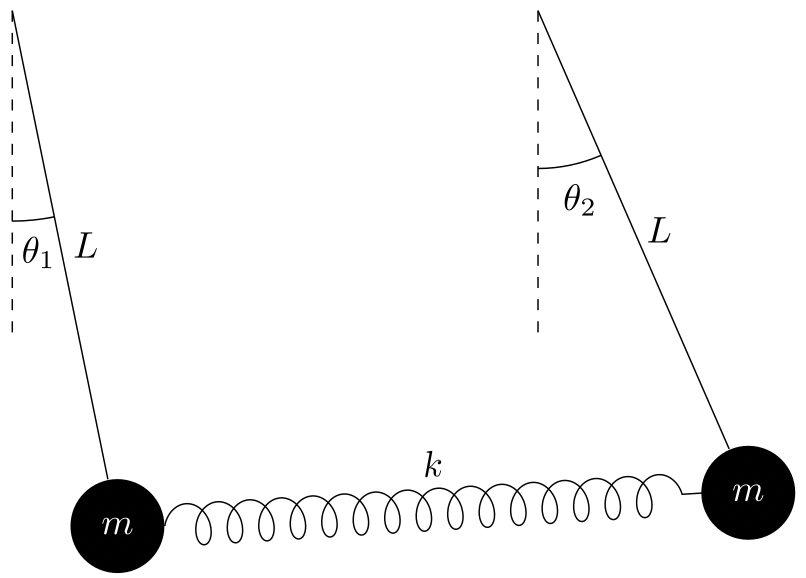
\includegraphics[width = 0.5\textwidth]{images/Pendulum.png}
        \caption{Сопряженный маятник}
        \label{fig:enter-label}
    \end{figure}

    Система состоит из двух математических маятников длины L, массы m, соединенные пружиной с жесткостью k. Обобщенные координаты - $\theta_1$ и $\theta_2$. Рассматриваемые начальные условия: $\dot \theta_1(0) = \dot \theta_2(0) = 0$, $\theta_1(0) = \theta_{10}$, $\theta_2(0) = \theta_{20}$.
    
\end{frame}

%----------------------------------------------------------------------------------------------------------

\begin{frame}{Аналитическое решение}

    $$\text{E}_k = \frac{1}{2}m L^2 (\ddot \theta_1 + \ddot \theta_2)$$

    $$\text{E}_p = m g L (2 - \cos \theta_1 - \cos \theta_2) + \frac{1}{2} k L^2 (\theta_1 - \theta_2)^2$$

    $$L = \frac{1}{2}m L^2 (\ddot \theta_1 + \ddot \theta_2) - m g L (2 - \cos \theta_1 - \cos \theta_2) - \frac{1}{2} k L^2 (\theta_1 - \theta_2)^2$$

    Воспользуемся уравнением Лагранжа:

    $$\frac{d}{dt} L_{\dot \theta} - L_{\theta} = 0,\ \theta = \{\theta_1, \theta_2\}$$

\end{frame}

%----------------------------------------------------------------------------------------------------------
\begin{frame}{Аналитическое решение}

    \begin{equation*}
        \begin{cases}
            \ddot \theta_1 + \frac{g}{L} \sin \theta_1 + \frac{k}{m} (\theta_1 - \theta_2)\\
            \ddot \theta_2 + \frac{g}{L} \sin \theta_2 - \frac{k}{m} (\theta_1 - \theta_2)
        \end{cases}
    \end{equation*}

    При малых углах получаем:

    \begin{equation*}
        \begin{cases}
            \ddot \theta_1 + \ddot \theta_2 + \frac{g}{L} (\theta_1 + \theta_2) = 0\\
            \ddot \theta_1 - \ddot \theta_2 + (\frac{g}{L} + 2 \frac{k}{m}) (\theta_1 - \theta_2) = 0
        \end{cases}
    \end{equation*}

    В итоге получаем:

    \begin{equation*}
        \begin{cases}
            \theta_1 = \frac{1}{2} (\theta_1(0) + \theta_2(0)) \cos (w_1 t) + \frac{1}{2} (\theta_1(0) - \theta_2(0)) \cos (w_2 t)\\
            \theta_1 = \frac{1}{2} (\theta_1(0) + \theta_2(0)) \cos (w_1 t) - \frac{1}{2} (\theta_1(0) - \theta_2(0)) \cos (w_2 t)
        \end{cases}
    \end{equation*}

    где $w_1 = \sqrt{\frac{g}{L}}$, $w_2 = \sqrt{\frac{g}{L} + 2 \frac{k}{m}}$.

\end{frame}

%----------------------------------------------------------------------------------------------------------

\begin{frame}{Эксперимент}

    Преобразуем систему: $x_1 = \theta_1 + \theta_2$, $y_1 = \dot x_1$, $x_2 = \theta_1 - \theta_2$, $y_2 = \dot x_2$.

    \begin{equation*}
        \begin{cases}
            \dot y_1 = - \frac{g}{L} x_1\\
            \dot x_1 = y_1\\
            \dot y_2 = - (\frac{g}{L} + 2 \frac{k}{m}) x_1\\
            \dot x_2 = y_2
        \end{cases}
    \end{equation*}

    \textbf{Начальные условия:} $\dot \theta_1(0) = \dot \theta_2(0) = 0$, $\theta_1(0) = 0.1 \text{рад}$, $\theta_2(0) = 0.05 \text{рад}$. 
    
    \textbf{Параметры:} $g = 9.81 \frac{\text{м}}{\text{с}^2}$, $L = 1 \text{м}$, $m = 1 \text{кг}$, $k = 40 \frac{\text{Н}}{\text{м}}$.

    \textbf{Модель:} Линейная + Тангенс + Линейная (как в семинаре).
    
\end{frame}

%----------------------------------------------------------------------------------------------------------

\begin{frame}{Результат}

    \begin{figure}
        \centering
        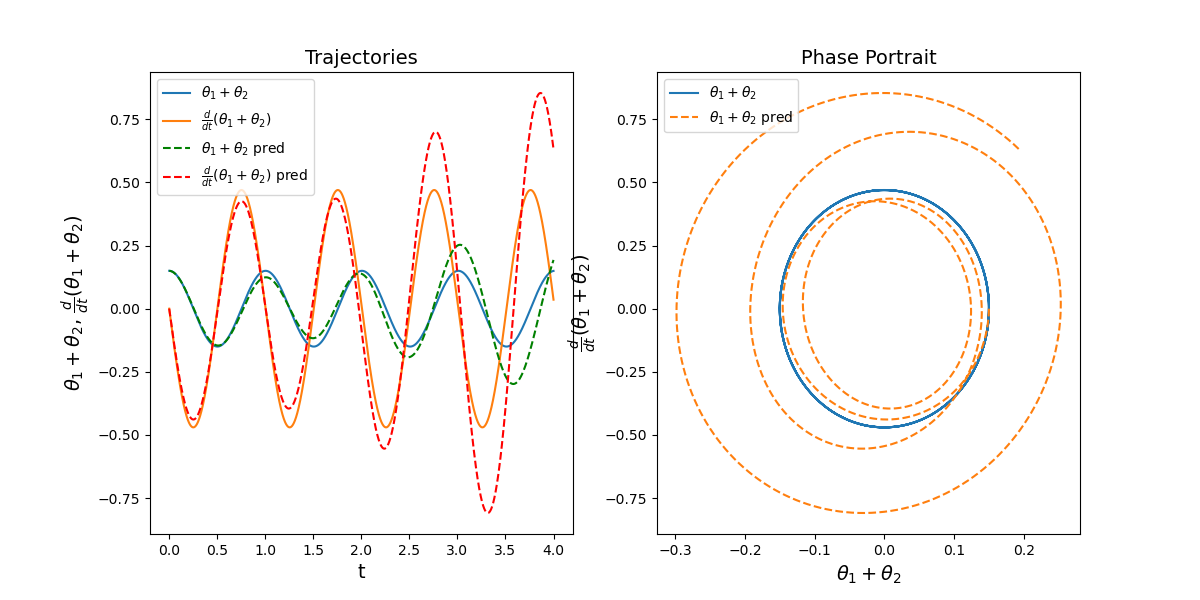
\includegraphics[width = 1 \textwidth]{images/Graph_sum.png}
        \caption{$\theta_1 + \theta_2$}
    \end{figure}

\end{frame}

%----------------------------------------------------------------------------------------------------------

\begin{frame}{Результат}

    \begin{figure}
        \centering
        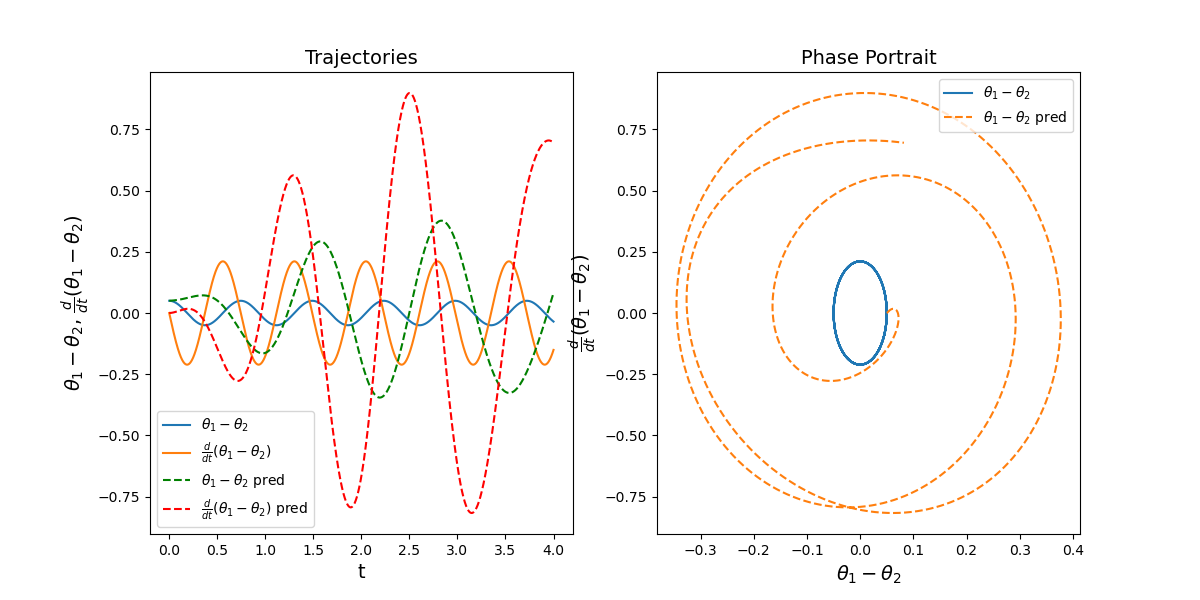
\includegraphics[width = 1 \textwidth]{images/Graph_difference.png}
        \caption{$\theta_1 - \theta_2$}
    \end{figure}
  
\end{frame}

%----------------------------------------------------------------------------------------------------------

\begin{frame}{Результат}

    \begin{figure}
        \centering
        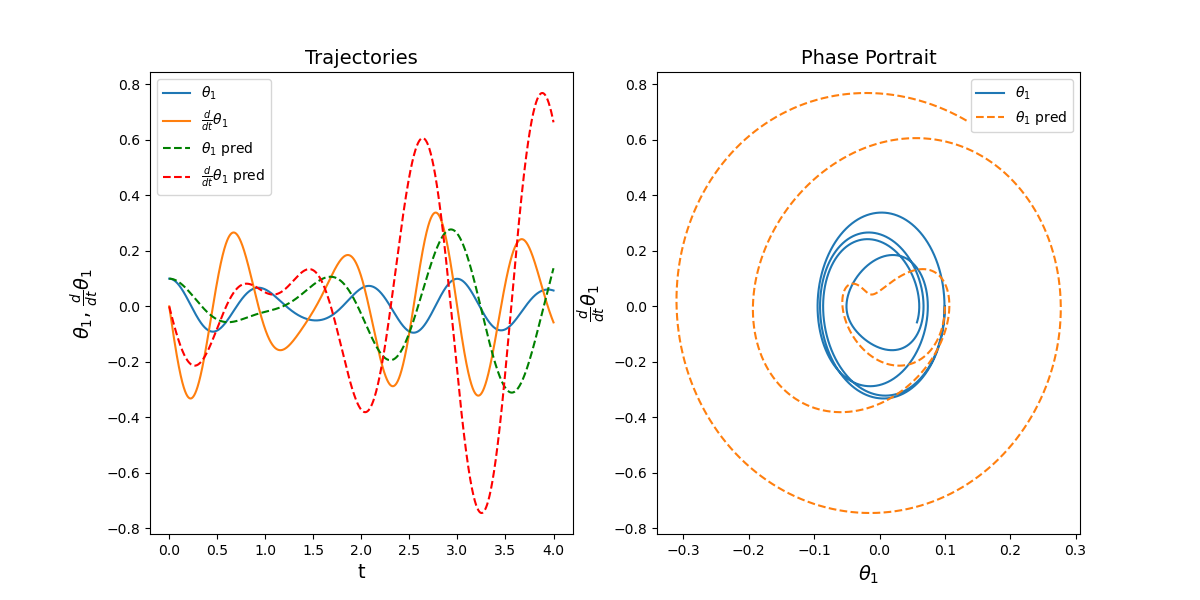
\includegraphics[width = 1 \textwidth]{images/Graph_1.png}
        \caption{$\theta_1$}
    \end{figure}

\end{frame}

%----------------------------------------------------------------------------------------------------------

\begin{frame}{Результат}

    \begin{figure}
        \centering
        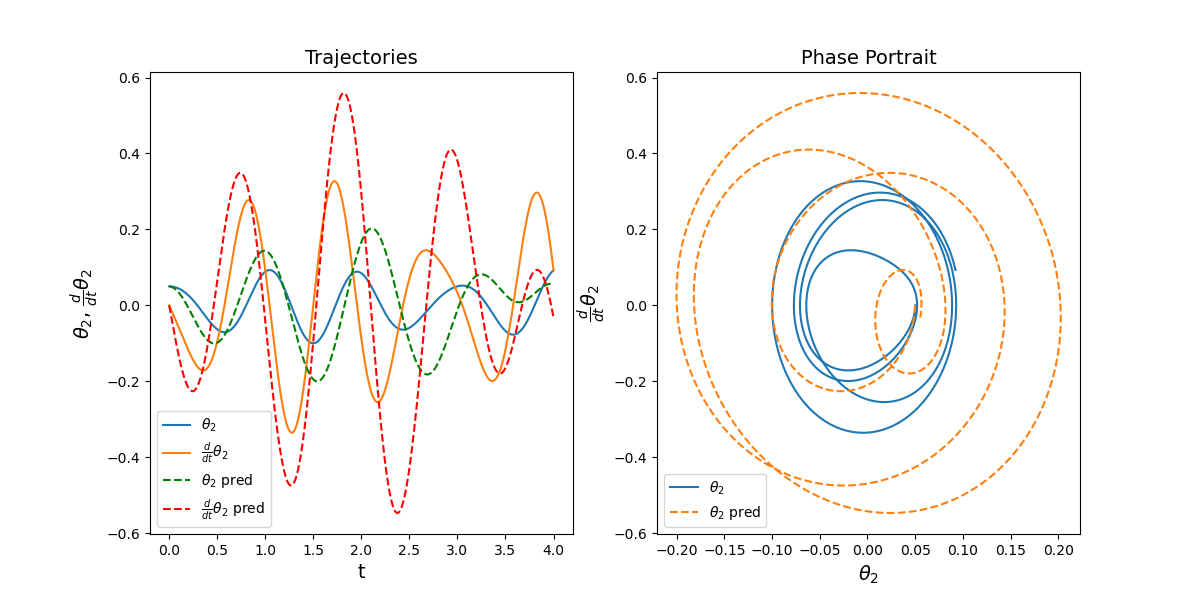
\includegraphics[width = 1 \textwidth]{images/Graph_2.png}
        \caption{$\theta_2$}
    \end{figure}
  
\end{frame}

%----------------------------------------------------------------------------------------------------------

\begin{frame}{Выводы}
    \begin{itemize}
        \item Модель может с хорошей точностью предсказывать только для случаев, когда осцилляции не очень большие и время не очень большое;
        \item SGD не работает, Adam работает, но очень тяжело подобрать шаг, так как либо модель находится в минимуме, либо вылетает на бесконечность;
        \item Код \url{https://github.com/Dd0-s/Mathematical_forecasting_methods}
    \end{itemize}
\end{frame}

%----------------------------------------------------------------------------------------------------------

\end{document}